w\subsection{CT Periodic FS and LTI systems}
\begin{definition}
    
\end{definition}

\begin{derivation}
    \begin{enumerate}
        \item \textbf{Recall:} For \( s \in \mathbb{C} \):

        \begin{center}
            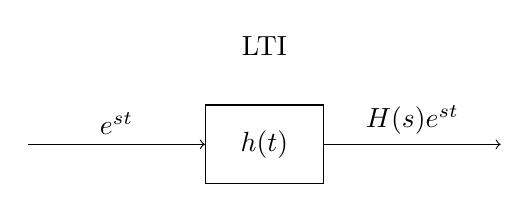
\begin{tikzpicture}
                \node at (0,0) [draw, rectangle, minimum width=1.5cm, minimum height=1cm] (H) {$h(t)$};
                \draw[->] (-3,0) -- (H) node[midway, above] {$e^{st}$};
                \draw[->] (H) -- (3,0) node[midway, above] {$H(s) e^{st}$};
                \node[above] at (0,1) {LTI};
            \end{tikzpicture}
        \end{center}
        \begin{itemize}
            \item \textbf{Eigenfunction:} $e^{st}$
            \item \textbf{Eigenvalue:} $H(s)$
            \item \textbf{System function, also called 2-sided Laplace Transform:} $H(s) = \int_{-\infty}^{\infty} h(\tau) e^{-s \tau} \, d\tau$ 
        \end{itemize}

        \item \textbf{If we specify} \( s = j \omega = j 2 \pi f \):

        \begin{center}
            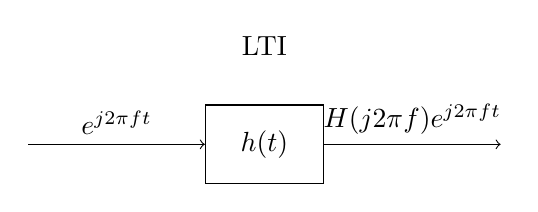
\begin{tikzpicture}
                \node at (0,0) [draw, rectangle, minimum width=1.5cm, minimum height=1cm] (H) {$h(t)$};
                \draw[->] (-3,0) -- (H) node[midway, above] {$e^{j 2 \pi f t}$};
                \draw[->] (H) -- (3,0) node[midway, above] {$H(j 2 \pi f) e^{j 2 \pi f t}$};
                \node[above] at (0,1) {LTI};
            \end{tikzpicture}
        \end{center}
        \begin{itemize}
            \item \textbf{Frequency response:} $H(j 2 \pi f) = \int_{-\infty}^{\infty} h(t) e^{-j 2 \pi f t} \, dt$
            \begin{itemize}
                \item This is the Fourier Transform of \( h(t) \), a special case of the Laplace Transform along the imaginary axis.
            \end{itemize}
        \end{itemize}

        \item Suppose input \( T \)-periodic:

        \begin{center}
            \begin{tikzpicture}
                \node at (0,0) [draw, rectangle, minimum width=1.5cm, minimum height=1cm] (H) {$h(t)$};
                \draw[->] (-3,0) -- (H) node[midway, above] {$x$};
                \draw[->] (H) -- (3,0) node[midway, above] {$y = x * h$};
                \node[above] at (0,1) {LTI};
            \end{tikzpicture}
        \end{center}
        \begin{itemize}
            \item \textbf{Input:} $ x \underset{T}{\overset{FS}{\leftrightarrow}} c_k \; \therefore \; x(t) = \sum_{k \in \mathbb{Z}} c_k e^{j 2 \pi \frac{k}{T} t}$
            \begin{itemize}
                \item \( |k| > 1 \): \( k \)-th harmonic
                \item \( k = 0 \): DC component
                \item \( T \): fundamental frequency
            \end{itemize}
            \item \textbf{Output:} $y \underset{T}{\overset{FS}{\leftrightarrow}} H\left( j 2 \pi \frac{k}{T} \right) c_k \; \therefore \; y(t) = \sum_{k \in \mathbb{Z}} H\left( j 2 \pi \frac{k}{T} \right) c_k e^{j 2 \pi \frac{k}{T} t}$ 
        \end{itemize}
    \end{enumerate}
\end{derivation}

\begin{example}
    The Fourier Transform \( H(j 2 \pi f) \) of \( h(t) = e^{-t} u(t) \) is given by:

    \begin{align*}
        H(j 2 \pi f) &= \int_{0}^{\infty} h(t) e^{-j 2 \pi f t} \, dt \\
        &= \int_{0}^{\infty} e^{-t} e^{-j 2 \pi f t} \, dt \\
        &= \int_{0}^{\infty} e^{(-1 + j 2 \pi f)t} \, dt \\
        &= \left[ \frac{e^{(-1 + j 2 \pi f)t}}{-1 + j 2 \pi f} \right]_{0}^{\infty} \\
        &= \frac{0 - 1}{-1 + j 2 \pi f} \\
        &= \frac{1}{1 + j 2 \pi f}
    \end{align*}

    Thus,
    \begin{equation*}
        H(j 2 \pi f) = \frac{1}{1 + j 2 \pi f}
    \end{equation*}

    \begin{center}
        \begin{tikzpicture}
            \draw[->] (0,0) -- (3.5,0) node[right] {$t$};
            \draw[->] (0,0) -- (0,2.5) node[above] {};
            \node[above left] at (0,2) {$1$};
            \node[below left] at (0,0) {$0$};
            \draw[thick, domain=0:3.2, samples=100] plot (\x,{e^(-\x)});
        \end{tikzpicture}
    \end{center}

    If \( x \underset{T}{\overset{FS}{\leftrightarrow}} c_k \), then the output \( y = x * h \) has the Fourier Series coefficients:

    \begin{equation*}
        y \underset{T}{\overset{FS}{\leftrightarrow}} \frac{c_k}{1 + j 2 \pi \frac{k}{T}}
    \end{equation*}
    \begin{itemize}
        \item RC Filter.
    \end{itemize}

\end{example}

\subsection{DT Periodic FS and LTI systems}
\begin{definition}
    
\end{definition}

\begin{derivation}
    \begin{enumerate}
        \item Similarly, in discrete time, let \( z = e^s \), \( s \in \mathbb{C} \):

        \begin{center}
            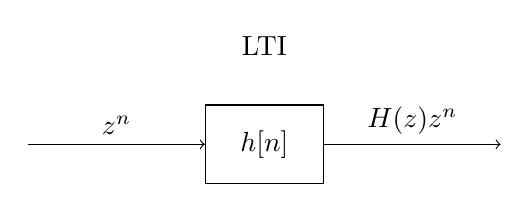
\begin{tikzpicture}
                \node at (0,0) [draw, rectangle, minimum width=1.5cm, minimum height=1cm] (H) {$h[n]$};
                \draw[->] (-3,0) -- (H) node[midway, above] {$z^n$};
                \draw[->] (H) -- (3,0) node[midway, above] {$H(z) z^n$};
                \node[above] at (0,1) {LTI};
            \end{tikzpicture}
        \end{center}
        \begin{itemize}
            \item \textbf{Z-transform:} $H(z) = \sum_{k \in \mathbb{Z}} h[k] z^{-k}$
        \end{itemize}
        
        \item \textbf{Now, if} \( s = j 2 \pi f \), \textbf{then} \( z = e^{j 2 \pi f} \):
        
        \begin{center}
            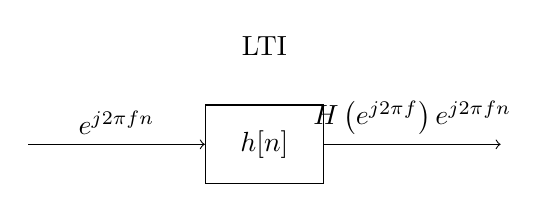
\begin{tikzpicture}
                \node at (0,0) [draw, rectangle, minimum width=1.5cm, minimum height=1cm] (H) {$h[n]$};
                \draw[->] (-3,0) -- (H) node[midway, above] {$e^{j 2 \pi f n}$};
                \draw[->] (H) -- (3,0) node[midway, above] {$H\left( e^{j 2 \pi f} \right) e^{j 2 \pi f n}$};
                \node[above] at (0,1) {LTI};
            \end{tikzpicture}
        \end{center}
        \begin{itemize}
            \item \textbf{Frequency response:} $ H\left( e^{j 2 \pi f} \right) = \sum_{n \in \mathbb{Z}} h[n] e^{-j 2 \pi f n}$
        \end{itemize}
        
        \item For \( x \in \mathbb{P}^N \):
        
        \begin{center}
            \begin{tikzpicture}
                \node at (0,0) [draw, rectangle, minimum width=1.5cm, minimum height=1cm] (H) {$h[n]$};
                \draw[->] (-3,0) -- (H) node[midway, above] {$x$};
                \draw[->] (H) -- (3,0) node[midway, above] {$y = x * h$};
                \node[above] at (0,1) {LTI};
            \end{tikzpicture}
        \end{center}
        \begin{itemize}
            \item \textbf{Input:} $x \underset{N}{\overset{FS}{\leftrightarrow}} c_k, \; \therefore \; x = \sum_{k=0}^{N-1} c_k e^{j 2 \pi \frac{k}{N} n}$
            \item \textbf{Output:} $y \underset{N}{\overset{FS}{\leftrightarrow}} H\left( e^{j 2 \pi \frac{k}{N}} \right) c_k \; \therefore \; y[n] = \sum_{k=0}^{N-1} c_k H\left( e^{j 2 \pi \frac{k}{N}} \right) e^{j 2 \pi \frac{k}{N} n}$
        \end{itemize}
    \end{enumerate}
\end{derivation}